
\noindent 
This unit covers the following ideas. In preparation for the quiz and exam, make sure you have a lesson plan containing examples that explain and illustrate the following concepts.  
\begin{enumerate}
\item Describe uses for, and construct graphs of, space curves and parametric surfaces. Find derivatives of space curves, and use this to find velocity, acceleration, and find equations of tangent lines.
\item Describe uses for, and construct graphs of, functions of several variables. For functions of the form $z=f(x,y)$, this includes both 3D surface plots and 2D level curve plots.  For functions of the form $w=f(x,y,z)$, construct plots of level surfaces.
\item Describe uses for, and construct graphs of, vector fields and transformations.
\item If you are given a description of a vector field, curve, or surface (instead of a function or parametrization), explain how to obtain a function for the vector field, or a parametrization for the curve or surface.
\end{enumerate}
You'll have a chance to teach your examples to your peers prior to the exam.


\section{Function Terminology}
A function is a set of instructions involving two sets (called the domain and codomain).  A function assigns to each element of the domain $D$ exactly one element in the codomain $R$. We'll often refer to the codomain $R$ as the target space.  We'll write $$f\colon D\to R$$ when we want to remind ourselves of the domain and target space.  In this class, we will study what happens when the domain and target space are subsets of ${\mathbb{R}}^n$ (Euclidean $n$-space).  In particular, we will study functions of the form $$f\colon {\mathbb{R}}^n\to {\mathbb{R}}^m,$$ when $m$ and $n$ are 3 or less. The value of $n$ is the dimension of the input vector (or number of inputs).  The number $m$ is the dimension of the output vector (or number of outputs).  Our goal is to understand uses for each type of function, and be able to construct graphs to represent the function.

We will focus most of our time this semester on two- and three-dimensional problems. However, many problems in the real world require a higher number of dimensions. When you hear the word ``dimension'', it does not always represent a physical dimension, such as length, width, or height.  If a quantity depends on 30 different measurements, then the problem involves 30 dimensions.  As a quick illustration, the formula for the distance between two points depends on 6 numbers, so distance is really a 6-dimensional problem.  As another example, if a piece of equipment has a color, temperature, age, and cost, we can think of that piece of equipment being represented by a point in four-dimensional space (where the coordinate axes represent color, temperature, age, and cost).

% As we introduce each type of function, we'll introduce it in the context of a somewhat realistic setting.  
% After introducing each type of surface, we'll end this chapter with an assortment of functions to practice graphing.

\begin{problem}\label{pebble problem}%
\marginpar{See 
\href{https://sagecell.sagemath.org/?z=eJwrsS1LLNJQL1HXtOYqyMkv0TAz0TU00yqJM9JR0CjRMdAx0tQEAL5TCVo}{Sage}
or 
\href{http://wolfr.am/xoc07E}{Wolfram Alpha}. %http://www.wolframalpha.com/input/?i=f%28t%29%3D64-16t^2
Follow the links to Sage or Wolfram Alpha in all the problems below to see how to get the computer to graph the function.}%
A pebble falls from a 64 ft tall building.  Its height (in ft) above the ground $t$ seconds after it drops is given by the function $y=f(t)=64-16t^2$. What are $n$ and $m$ when we write this function in the form  $f\colon {\mathbb{R}}^n\to {\mathbb{R}}^m$? Construct a graph of this function.  How many dimensions do you need to graph this function?
\end{problem}

\section{Parametric Curves: $\vec f\colon \RR \to \RR^m$}

\begin{problem}\label{parametric curve in plane example}%
\marginpar{See \href{https://sagecell.sagemath.org/?z=eJwrsS1LLNJQL1HX5CpILErMTS0pykyOL8jJL9GINtJKzi_WKNHUUTDWKs7MA7JidRQ0SnQMdIy0CjI1NQFWdRJT}{Sage} or \href{http://wolfr.am/wAkR8l}{Wolfram Alpha}. %http://www.wolframalpha.com/input/?i=parametric+plot+%282+cos+t,+3+sin+t%29
See also Chapter 3 of this problem set.
 \bmw{There's a lot more practice of this idea in 11.1. You'll also find more practice in 13.1: 1-8.}}%
\larsonfive{\marginpar{See also Larson 10.2.  You can also find more practice in 12.1 and 12.3.}}%
A horse runs around an elliptical track. Its position at time $t$ is given by the  function $\vec r(t)=(2\cos t, 3\sin t).$ We could alternatively write this as $x=2\cos t, y=3\sin t$. 
 \begin{enumerate}
  \item What are $n$ and $m$ when we write this function in the form  $\vec r\colon {\mathbb{R}}^n\to {\mathbb{R}}^m$?
  \item Construct a graph of this function. 
  \item Next to a few points on your graph, include the time $t$ at which the horse is at this point on the graph. Include an arrow for the horse's direction.
  \item How many dimensions do you need to graph this function?
 \end{enumerate}
\end{problem}


Notice in the problem above that we placed a vector symbol above the function name, as in $\vec r\colon {\mathbb{R}}^n\to {\mathbb{R}}^m$.  When the target space (codomain) is 2-dimensional or larger, we place a vector above the function name to remind us that the output is more than just a number.

\begin{problem}%
\marginpar{See \href{https://sagecell.sagemath.org/?z=eJwNxksKgCAUBdB5q3Dmh2eQfWZuJXmIgpAodtt_Dg6crKC92g1IXIfdLoPb6aXz4JowSgz9aVCZhAJZt540aRL89hQRBqM0L_lDq7NR6h-iAhhm}{Sage} or \href{http://wolfr.am/ynm3kD}{Wolfram Alpha}. %http://www.wolframalpha.com/input/?i=parametric+plot+%283t,+64-16t^2%29
 \bmw{The text has more practice in 13.1: 1-8.}
\larsonfive{See also Larson 12.3.}}%
Consider the pebble from problem \ref{pebble problem}. The pebble's height was given by $y=64-16t^2$.  The pebble also has some horizontal velocity (it's moving at 3 ft/s to the right).  If we let the origin be the base of the 64 ft building, then the position of the pebble at time $t$ is given by $\vec r(t) = (3t, 64-16t^2)$.
 \begin{enumerate}
  \item What are $n$ and $m$ when we write this function in the form  $\vec r\colon {\mathbb{R}}^n\to {\mathbb{R}}^m$?
  \item At what time does the pebble hit the ground (the height reaches zero)?  Construct a graph of the pebble's path from when it leaves the top of the building till when it hits the ground.
  \item\marginpar{See Section~\ref{derivatives and tangent lines} and Definition~\ref{definition velocity acceleration}.}%
 Find the pebble's velocity and acceleration vectors at $t=1$? Draw these vectors on your graph with their base at the pebble's position at $t=1$. 
  \item At what speed is the pebble moving when it hits the ground?
 \end{enumerate}
\end{problem}

In the next problem, we keep the input as just a single number $t$, but the output is now a vector in $\mathbb{R}^3$.

\begin{problem}\label{jet intro for space curves}%
\label{space curve example}%
\marginpar{See \href{https://sagecell.sagemath.org/?z=eJxL0yjRtNUw0krOLwaydBSMtIoz88CsEk2ugsSixNzUkqLM5PiCnPwSjTQdBY0SHQMdBROtgkxNTQAYOxGO}{Sage} or \href{http://www.wolframalpha.com/input/?i=parametric+plot+3D++\%282+cos+t\%2C+2+sin+t\%2C+t\%29+for+t+from+0+to+4+pi}{Wolfram Alpha}. 
  \bmw{The text has more practice in 13.1: 9-14.}%
\larsonfive{More practice is in Larson 12.1:9--12, 21--24, 27--32.}}%
 A jet begins spiraling upwards to gain height. The position of the jet after $t$ seconds is modeled by the equation 
$\vec r(t)=(2\cos t, 2\sin t, t).$ We could alternatively write this as $x=2\cos t,\, y=2\sin t,\, z=t$. 
\begin{enumerate}
 \item What are $n$ and $m$ when we write this function in the form  $\vec r\colon {\mathbb{R}}^n\to {\mathbb{R}}^m$? 
 \item Construct a graph of this function by picking several values of $t$ and plotting the resulting points $(2\cos t, 2\sin t, t)$. 
 \item Next to a few points on your graph, include the time $t$ at which the jet is at this point on the graph. Include an arrow for the jet's direction.
 \item  How many dimensions do you need to graph this function?
\end{enumerate}
\end{problem}

In all the problems above, you should have noticed that in order to draw a function (provided you include arrows for direction, or use an animation to represent ``time''), you can determine how many dimensions you need to graph a function by just summing the dimensions of the domain and codomain. This is true in general.

\begin{problem}\marginpar{See Section~\ref{derivatives and tangent lines} and Definition~\ref{definition velocity acceleration}.}%
\marginpar{\bmw{The text has more practice in 13.1: 19-22.}\larsonfive{More practice in Larson 12.2:23--30.}}%
 Use the same set up as problem \ref{space curve example}, namely $$\vec r(t)=(2\cos t, 2\sin t, t).$$  You'll need a graph of this function to complete this problem.
 \begin{enumerate}
  \item Find the first and second derivative of $\vec r(t)$. 
  \item Compute the velocity and acceleration vectors at $t=\pi/2$. Place these vectors on your graph with their tails at the point corresponding to $t=\pi/2$.
  \item Give an equation of the tangent line to this curve at $t=\pi/2$.
 \end{enumerate}
\end{problem}


\section{Parametric Surfaces: $\vec f\colon  \RR^2 \to \RR^3$}
We now increase the number of inputs from 1 to 2.  This will allow us to graph many space curves at the same time.

\begin{problem} \label{parametric surface example}%
\marginpar{See \href{https://sagecell.sagemath.org/?z=eJxL0yjRUUjUtNVI1ErOL9Yo0QTytIoz88CsEk2ugsSixNzUkqLM5PiCnPwSjTQdBaAOAx0FE62CTKASjUQdBSMgT1OTCwBCiRSf}{Sage} or \href{http://www.wolframalpha.com/input/?i=parametric+plot+3D++\%28a+cos+t\%2C+a+sin+t\%2C+t\%29+for+t+from+0+to+4+pi+and+a+from+2+to+4}{Wolfram Alpha}.
\larsonfive{More practice in Larson 15.5:1--6.}}%
 The jet from problem \ref{jet intro for space curves} is actually accompanied by several jets flying side by side. As all the jets fly, they leave a smoke trail behind them (it's an air show). The smoke from one jet spreads outwards to mix with the neighboring jet, so that it looks like the jets are leaving a rather wide sheet of smoke behind them as they fly. The position of two of the many other jets is given by $\vec r_3(t)=(3\cos t, 3\sin t, t)$ and $\vec r_4(t)=(4\cos t,4\sin t,t)$.  A function which represents the smoke stream is $\vec r(a,t)=(a\cos t, a\sin t, t)$ for $0\leq t\leq 4\pi$ and $2\leq a\leq 4$.
 \begin{enumerate}
  \item What are $n$ and $m$ when we write the function $\vec r(a,t)=(a\cos t, a\sin t, t)$ in the form  $\vec r\colon {\mathbb{R}}^n\to {\mathbb{R}}^m$?
  \item Start by graphing the position of the three jets $\vec r(2,t)=(2\cos t, 2\sin t, t)$, $\vec r(3,t)=(3\cos t, 3\sin t, t)$ and $\vec r(4,t)=(4\cos t,4\sin t,t)$.  
  \item Let $t=0$ and graph the curve $r(a,0)=(a,0,0)$ for $a\in[2,4]$.  Then repeat this for $t=\pi/2,\pi,3\pi/2$.
  \item Describe the resulting surface.
 \end{enumerate}
\end{problem}

The function above is called a parametric surface.  Parametric surfaces are formed by joining together many parametric space curves. Most of 3D computer animation is done using parametric surfaces. Woody's entire body in {\it Toy Story} is a collection of parametric surfaces. Car companies create computer models of vehicles using parametric surfaces, and then use those parametric surfaces to study collisions. Often the mathematics behind these models is hidden in the software program, but parametric surfaces are at the heart of just about every 3D computer model.

\begin{problem}\label{second parametric surface example}%
\marginpar{See \href{https://sagecell.sagemath.org/?z=eJxL0yjVUSjTtNUo1UrOL9Yo09RRKNUqzsyDsOKMNLkKEosSc1NLijKT4wty8ks00nQUQHoMdBRMgEo0ynQMdIy0CjI1NQFPyxVa}{Sage} or \href{http://wolfr.am/A90cfW}{Wolfram Alpha}.% http://www.wolframalpha.com/input/?i=parametric+plot+3d+%28u+cos+v,+u+sin+v,+u^2%29
}%
 Consider the parametric surface $\vec r(u,v)=(u\cos v, u\sin v, u^2)$ for $0\leq u\leq 3$ and $0\leq v\leq 2 \pi$.
 Construct a graph of this function. To do so, let $u$ equal a constant (such as 1, 2, 3) and then graph the resulting space curve.  Then let $v$ equal a constant (such as 0, $\pi/2$, etc.) and graph the resulting space curve until you can visualize the surface. [Hint: Think satellite dish.] 
\end{problem}


\section{Functions of Several Variables: $f\colon \RR^n \to \RR$}

In this section we'll focus on functions of the form $f\colon \mathbb{R}^2\to\mathbb{R}^1$ and $f\colon \mathbb{R}^3\to\mathbb{R}^1$; we'll keep the output as a real number. In the next problem, you should notice that the input is a vector $(x,y)$ and the output is a number $z$. There are two ways to graph functions of this type.  The next two problems show you how. 

\begin{problem}\label{surface graph for a function of two variables}%
\marginpar{See \href{https://sagecell.sagemath.org/?z=eJxL06jQqdS0tdStiDPSrYwz4irIyS8xTtFI01EAyuga6xhrAlmVEJYmADAVC84}{Sage} or 
\href{http://wolfr.am/wny0IF}{Wolfram Alpha}.%http://www.wolframalpha.com/input/?i=plot+3d+9-x^2-y^2
}%
\larsonfive{\marginpar{See Larson 13.1:33--40.}}%
 A computer chip has been disconnected from electricity and sitting in cold storage for quite some time.  The chip is connected to power, and a few moments later the temperature (in Celsius) at various points $(x,y)$ on the chip is measured. From these measurements, statistics is used to create a temperature function $z=f(x,y)$ to model the temperature at any point on the chip. Suppose that this chip's temperature function is given by the equation $z=f(x,y)=9-x^2-y^2$. We'll be creating a 3D model of this function in this problem, so you'll want to place all your graphs on the same $x,y,z$ axes.
\begin{enumerate}
 \item What is the temperature at $(0,0)$, $(1,2)$, and $(-4,3)$? \marginpar{\bmw{See 14.1: 1-4.}}
 \item If you let $y=0$, construct a graph of the temperature $z=f(x,0) = 9-x^2-0^2$, or just $z=9-x^2$. In the $xz$ plane (where $y=0$) draw this upside down parabola.
 \item Now let $x=0$. Draw the resulting parabola in the $yz$ plane.
 \item Now let $z=0$. Draw the resulting curve in the $xy$ plane.
 \item Once you've drawn a curve in each of the three coordinate planes, it's useful to pick an input variable (either $x$ or $y$) and let it equal various constants. So now let $x=1$ and draw the resulting parabola in the plane $x=1$.  Then repeat this for $x=2$.
 \item Describe the shape. Add any extra features to your graph to convey the 3D image you are constructing. \marginpar{\bmw{See 14.1: 37-48.}}
\end{enumerate}
\end{problem}

\begin{problem}\label{cake level curves plot}%
\marginpar{See \href{https://sagecell.sagemath.org/?z=eJydj81qwzAQhO9-iiWXWCCHJqbQHHTtExR6KI1RnBVWWWuNVibR21fOH_Ta2-7M7PCtqy86K7NvLoddkw-7aiJO7al2GorTtLpVZcq3SW1k4HOtqiGNVK8-EZY0pDPDyTuHEUMCSZlQgB30HBLP8RoSEIbMM_Q2gCCWdcQllAb8EwSekucgm5Wq7nq36IXoCfTg0Y9LMV8veqtf9Zvefy8qcTzaaD7ijLof7WTWP5jWT_7_FpM9IsmtFpwnMu-WBPVV73wgH_DuWpmwT1205RuzVdUvSwN0NA}{Sage} or 
\href{http://wolfr.am/wny0IF}{Wolfram Alpha}.%http://www.wolframalpha.com/input/?i=plot+3d+9-x^2-y^2
}%
\larsonfive{\marginpar{See Larson 13.1:45--56.}}%
We'll be using the same function $z=f(x,y)=9-x^2-y^2$ as the previous problem.  However, this time we'll construct a graph of the function by only studying places where the temperature is constant.  We'll create a graph in 2D of the surface (similar to a topographical map). 
 \begin{enumerate}
  \item%
\marginpar{\bmw{See 14.1: 13-16 and 31-36.}}%
Which points in the plane have zero temperature? Just let $z=0$ in $z=9-x^2-y^2$. Plot the corresponding points in the $xy$-plane, and write $z=0$ next to this curve. This curve is called a level curve. As long as you stay on this curve, your temperature will remain level, it will not increase nor decrease. 
  \item Which points in the plane have temperature $z=5$?  Add this level curve to your 2D plot and write $z=5$ next to it.
  \item Repeat the above for $z=8$, $z=9$, and $z=1$. What's wrong with letting $z=10$? \marginpar{\bmw{See 14.1: 37-48.}}
  \item Using your 2D plot, construct a 3D image of the function by lifting each level curve to its corresponding height.
 \end{enumerate}
\end{problem}

\begin{definition}
 A level curve of a function $z=f(x,y)$ is a curve in the $xy$-plane found by setting the output $z$ equal to a constant. Symbolically, a level curve of $f(x,y)$ is the curve $c=f(x,y)$ for some constant $c$.  A 2D plot consisting of several level curves is called a contour plot of $z=f(x,y)$.
\end{definition}

\begin{problem}%

\marginpar{See \href{https://sagecell.sagemath.org/?z=eJxL06jQqdS0rdCtjDPiKs7IL9coyMkvMU7RSNNRAErpGusYawJZlRCWpiZETXJ-Xkl-aVE8SC12lToKybmJBbbqWakl6kB2fk5-UVJikW1IUWmqTk5iUmpOMZitqQkAhh0mmg}{Sage} or 
\href{http://wolfr.am/wBOk1b}{Wolfram Alpha}.%http://www.wolframalpha.com/input/?i=plot+3d+x-y^2
\bmw{More practice is in 14.1: 37-48.}}%
\larsonfive{\marginpar{See Larson 13.1:45--56.}}%
 Consider the function $f(x,y)=x-y^2$.
\begin{enumerate}
 \item Construct a 3D surface plot of $f$. [So just graph in 3D the curves given by $x=0$ and $y=0$ and then try setting $x$ or $y$ equal to some other constants, like $x=1$, $x=2$, $y=1$, $y=2$, etc.]
 \item Construct a contour plot of $f$. [So just graph in 2D the curves given by setting $z$ equal to a few constants, like $z=0$, $z=1$, $z=-4$, etc.]
 \item% 
\marginpar{\bmw{See 14.1: 49-52.}}%
Which level curve passes through the point $(2,2)$?  Draw this level curve on your contour plot.
\end{enumerate}
\end{problem}

Notice that when we graphed the previous two functions (of the form $z=f(x,y)$) we could either construct a 3D surface plot, or we could reduce the dimension by 1 and construct a 2D contour plot by letting the output $z$ equal various constants. 
The next function is of the form $w=f(x,y,z)$, so it has 3 inputs and 1 output.  We could write $f\colon \mathbb{R}^3\to\mathbb{R}^1$. We would need 4 dimensions to graph this function, but graphing in 4D is not an easy task.  Instead, we'll reduce the dimension and create plots in 3D to describe the level surfaces of the function.

\begin{problem}%
\marginpar{See \href{https://sagecell.sagemath.org/?z=eJwrSyzSUK_QqdSpUtfkCtEAszRtDQ0MdCvijHQrgbgqzogrM7cgJzM5syS-ICe_xDhFA67Q1tJSRwHIUdA11lEw1gSyK8FsMLMKytRUAADtWRrw}{Sage}.  Wolfram Alpha currently does not support drawing level surfaces.  You could also use Mathematica or \href{http://demonstrations.wolfram.com/LevelSurfacesAndQuadraticSurfaces/}{Wolfram Demonstrations}.

\bmw{You can access more problems on drawing level surfaces in 12.6:1-44 or 14.1:53-60.}}%
\larsonfive{\marginpar{See Larson 11.6 and 13.1:69--74, as well as 13.1, Example 6.}}%
 Suppose that an explosion occurs at the origin $(0,0,0)$. Heat from the explosion starts to radiate outwards.  Suppose that a few moments after the explosion, the temperature at any point in space is given by $w=T(x,y,z)=100-x^2-y^2-z^2.$ 
\begin{enumerate}
 \item Which points in space have a temperature of 99?  To answer this, replace $T(x,y,z)$ by $99$ to get $99=100-x^2-y^2-z^2$. Use algebra to simplify this to $x^2+y^2+z^2=1$.  Draw this object.
 \item Which points in space have a temperature of 96? of 84? Draw the surfaces. 
 \item What is your temperature at $(3,0,-4)$? Draw the level surface that passes through $(3,0,-4)$.
\item The 4 surfaces you drew above are called level surfaces. If you walk along a level surface, what happens to your temperature?
 \item As you move outwards, away from the origin, what happens to your temperature?
\end{enumerate}
\end{problem}

\note{Talk about graphing functions with 4 or more variables.  Show the class \href{http://www.osirix-viewer.com/}{OsiriX} as an example of graphing a 4d function (where opacity is the density of material.  Also, practice sliding a plane through a 3d object to get an idea of what the contour plots are telling us.}

\begin{problem}
\marginpar{See \href{https://sagecell.sagemath.org/?z=eJwrSyzSUK_QqdSpUtfkStMAszRtK-KMtKvijLgycwtyMpMzS-ILcvJLjFM04ApsTXQUgGwFXWMdBWNNILsSzAYzq6BMTQUAEvYY4A}{Sage}.}%
\larsonfive{\marginpar{See Larson 11.6:7--16.}}%
Consider the function $w=f(x,y,z)=x^2+z^2$. This function has an input $y$, but notice that changing the input $y$ does not change the output of the function.
 \begin{enumerate}
  \item Draw a graph of the level surface $w=4$. [When $y=0$ you can draw one curve.  When $y=1$, you should draw the same curve.  When $y=2$, again you draw the same curve.  This kind of graph is called a cylinder, and is important in manufacturing where you extrude an object through a hole.]
  \item Graph the surface $9=x^2+z^2$ (so the level surface $w=9$).
  \item Graph the surface $16=x^2+z^2$.
 \end{enumerate}
\end{problem}

Most of our examples of function of the form $w=f(x,y,z)$ can be drawn by using our knowledge about conic sections. We can graph ellipses and hyperbolas if there are only two variables. So the key idea is to set one of the variables equal to a constant and then graph the resulting curve.  Repeat this with a few variables and a few constants, and you'll know what the surface is. Sometimes when you set a specific variable equal to a constant, you'll get an ellipse. If this occurs, try setting that variable equal to other constants, as ellipses are generally the easiest curves to draw.

\begin{problem}\marginpar{See \href{https://sagecell.sagemath.org/?z=eJwrSyzSUK_QqdSpUtfkStMAszRtK-KMdCvjjLSr4oy4MnMLcjKTM0viC3LyS4xTNOCKbA11FIBsBV1jHQVjTSC7EswGM6ugTE0FAIXAGhM}{Sage}.  \bmw{Remember you can find more practice in 12.6:1-44 or 14.1: 53-64.}}%
\larsonfive{\marginpar{See Larson 11.6 and 13.1:69--74, as well as 13.1, Example 6.}}%
 Consider the function $w=f(x,y,z)=x^2-y^2+z^2$.\marginparbmw{We'll have a few people present this problem.}
 \begin{enumerate}
  \item Draw a graph of the level surface $w=1$. [You need to graph $1=x^2-y^2+z^2$. Let $x=0$ and draw the resulting curve. Then let $y=0$ and draw the resulting curve. Let either $x$ or $y$ equal some more constants (whichever gave you an ellipse), and then draw the resulting ellipses.]  
  \item Graph the level surface $w=4$. [Divide both sides by $4$ (to get a 1 on the left) and the repeat the previous part.]
  \item Graph the level surface $w=-1$. [Try dividing both sides by a number to get a 1 on the left. If $y=0$ doesn't help, try $y=1$ or $y=2$.]
  \item Graph the level surface that passes through the point $(3,5,4)$. [Hint: what is $f(3,5,4)$?]
 \end{enumerate}
\end{problem}

\section{Vector Fields and Transformations: $\vec f\colon \RR^n\to\RR^n$}

We've covered the following types of functions in the problems above.
\begin{itemize}
 \item $y=f(x)$ or $f\colon \mathbb{R}\to\mathbb{R}$ (functions of a single variable)
 \item $\vec r(t)=(x,y)$ or $f\colon \mathbb{R}\to\mathbb{R}^2$ (parametric curves)
 \item $\vec r(t)=(x,y,z)$ or $f\colon \mathbb{R}\to\mathbb{R}^3$ (space curves)
 \item $\vec r(u,v)=(x,y,z)$ or $f\colon \mathbb{R}^2\to\mathbb{R}^3$ (parametric surfaces)
 \item $z=f(x,y)$ or $f\colon \mathbb{R}^2\to\mathbb{R}$ (functions of two variables)
 \item $z=f(x,y,z)$ or $f\colon \mathbb{R}^3\to\mathbb{R}$ (functions of three variables)
\end{itemize}
This section We will consider functions from $\mathbb{R}^2$ to $\mathbb{R}^2$ and functions from $\mathbb{R}^3$ to $\mathbb{R}^3$.  Depending on the application, we may view these functions as either transformations of 2D or 3D space, or we may view them as vector fields in the plane or space.


\subsection{Vector Fields}

A vector field $\vec F(x,y)=(M,N)$ is visualized by putting the vector $(M,N)$ at the point $(x,y)$, so you end up with a picture with a lot of vectors.  These are often used to visualize flows of air or liquids.  For example, see \href{http://ccom.unh.edu/vislab/projects/2d_flow_vis.html}{VisLab}, the \href{http://nowcoast.noaa.gov/}{NOAA visualizations},  \href{http://artsci.drake.edu/urness/research.html}{Tim Urness's research page}, or the \href{http://www.nsf.gov/news/special_reports/scivis/}{International Visualization Challenge}.  There are also lots of other visualizations challenges.  Figuring out how to convey information in an asthetic and effective way is a tough challenge.

\begin{problem}%
\marginpar{See 
\href{https://sagecell.sagemath.org/?z=eJxz06jQqdRUsFXQMNKq0K7UqdA20qrU5CrIyS-JL0tNLskvik_LTM1J0XDTUQAq1TU00DE00ASyK2FsTQCKaxIN}{Sage} or
\href{http://wolfr.am/y4gIgX}{Wolfram Alpha}. % http://www.wolframalpha.com/input/?i=plot+a+vector+field&f1={2x%2By%2Cx%2B2y}&x=6&y=7&f=VectorPlot.vectorfunction_{2x%2By%2Cx%2B2y}&f2=x&f=VectorPlot.vectorplotvariable1_x&f3=-10&f=VectorPlot.vectorplotlowerrange1_-10&f4=10&f=VectorPlot.vectorplotupperrange1_10&f5=y&f=VectorPlot.vectorplotvariable2_y&f6=-10&f=VectorPlot.vectorplotlowerrange2_-10&f7=10&f=VectorPlot.vectorplotupperrange2_10
The computer will shrink the largest vector down in size so it does not overlap any of the others, and then reduce the size of all the vectors accordingly. \bmw{See 16.2: 39-44 for more practice.}}%
\larsonfive{\marginpar{See Larson 15.1:1--19.}}%
 Consider the vector field $\vec F(x,y)=(2x+y,x+2y)$.  In this problem, you will construct a graph of this vector field by hand.
\begin{enumerate}
 \item Compute $\vec F(1,0)$. Then draw the vector $F(1,0)$ with its base at $(1,0)$.
 \item Compute $\vec F(1,1)$. Then draw the vector $F(1,1)$ with its base at $(1,1)$.
 \item Repeat the above process for the points $(0,1)$, $(-1,1)$, $(-1,0)$, $(-1,-1)$, $(0,-1),$ and $(1,-1)$. Remember, at each point draw a vector.  
\end{enumerate}
\end{problem}


\begin{problem}[Spin field]\marginpar{Change the Sage code in the link above to get the computer to plot this to check your work.  \bmw{See 16.2: 39-44 for more practice.}}%
\larsonfive{\marginpar{See Larson 15.1:1--19.}}%
 Consider the vector field $\vec F(x,y)=(-y,x)$. Construct a graph of this vector field. Remember, the key to plotting a vector field is ``at the point $(x,y)$, draw the vector $\vec F(x,y)$ with its base at $(x,y)$.''  Plot at least 8 vectors (a few in each quadrant), so we can see what this field is doing.
\end{problem}

\note{Talk about vector field visualization, mention line integral convolutions and streamline plots.  Show Sage or mathematica doing these sorts of plots.}

\marginpar{See \href{https://sagecell.sagemath.org/?z=eJxz06jQqdSp0lSwVdAA0joVmlwFOfkl8WWpySX5RfFpmak5KcYpGm46CkCFusY6xpo6IIUQlkYVhKEJAOGFExs}{Sage}.} We can also visualize 3d vector fields like $\vec F(x,y,z)=(y,z,x)$. \note{use 3d glasses and Sage/JMol's ability to render for 3d glasses to \emph{really} see this vector field!}

\subsection{Transformations}
\note{Make the transformations part a new chapter, along with the polar coordinate things they should know.}

Coordinate transformations let us view or discuss the plane or space in a different way.  A 2d transformation $\vec T(u,v)=(x,y)$ tells us how to transform a $(u,v)$ axes into an $(x,y)$ axes---the two outputs of $\vec T$ are considered the $x$ and $y$ coordinates corresponding to the inputs $u$ and $v$.

\begin{problem} \label{polar coordinate transformation graph}\marginpar{For this problem, you are just drawing many parametric curves.}%
\marginpar{Click \href{http://artsci.drake.edu/grout/mathbox/examples/polar.html}{here} or \href{http://artsci.drake.edu/grout/mathbox/examples/polar2.html}{here} for some help visualizing this transformation.}%
\larsonfive{\marginpar{See Larson 10.5.}}%
Consider the coordinate transformation $$\vec T(r,\theta) = (r\cos\theta,r\sin\theta).$$  In other words, according to $\vec T$, $x=r\cos\theta$ and $y=r\sin\theta$.  This is called the \emph{polar coordinate} transformation.  We will talk more about this transformation in the next chapter.
\begin{enumerate}
\item Draw two 2D axes, one having horizontal axis $r$ and vertical axis $\theta$, and the other axes having horizontal axis $x$ and vertical axis $y$.  In the next few parts, we'll see how $\vec T$ will tell us how points on the $(r,\theta)$ axes transform to points on the $(x,y)$ axes.
\item Plot the point $(r,\theta)=(1,\pi/2)$ on the $(r,\theta)$ axes.  According to $\vec T$, this point is transformed to what $(x,y)$ point?  Plot this corresponding point on the $(x,y)$ axes.
\item\marginpar{See \href{https://sagecell.sagemath.org/?z=eJwtizEKwCAMAHdfETolkqG0s79wLyJCA62GmP_TwW53B5fR2O_mhRJarGPiMgaLU_pvFNSkO2wZLZ0EMjeGxUGLlbe5Sb30GY4rM6yVYWc4ogrRBx0PIJI=&lang=sage}{Sage} to check your answer.}  Plot the line segment $r=3$ (for $\theta\in [0,2\pi]$) on the $(r,\theta)$ axes.  Plot the corresponding points on the $(x,y)$ axes by letting $r=3$ in $\vec T$ and graphing $\vec T(3,\theta)=(3\cos\theta,3\sin\theta)$ for $\theta\in[0,2\pi]$ (hint: this is just a parametric curve, like we've been plotting).
\item\marginpar{See \href{https://sagecell.sagemath.org/?z=eJxljM0KwkAMhO99iqGnZA1Y_DnuW_QuSykY0DZk8_5YXNGCt_n5ZkZyifschTN5mtZKzQk8VV0-jjtzXQL9SJ7PDK29oOlf80az6fHyBXZRZ8XLcw7X6WaPNajNBQ0SDIJTMmXGAf_s7mmbuAxyZX4Bxl853w==&lang=sage}{Sage}.  Notice that you can add two plots together to draw them both.}%
 Plot the line segment $\theta=\pi/4$ (for $r\in[0,5]$) on the $(r,\theta)$ axes.  Plot the corresponding points on the $(x,y)$ axes by letting $\theta=\frac{\pi}{4}$ and then, on the same axes as above, add the graph of 
$\vec T\left(r,\frac{\pi}{4}\right)=\left(r\frac{\sqrt 2}{2},r \frac{\sqrt 2}{2}\right)$ for $r\in[0,5]$.
\item\marginpar{Use Sage to check your answer.} To the same axes as above, add the graphs of 
$\vec T(1,\theta), \vec T(2,\theta), \vec T(4,\theta)$  for $\theta\in[0,2\pi]$ and 
$\vec T(r,0), \vec T(r,\pi/2), \vec T(r,3\pi/4), \vec T(r,\pi)$ for $r\in[0,5]$. 
\end{enumerate}
\end{problem}

In the previous problem, you saw how we can think of 2D transformations as mapping the points of one plane onto another.  Another way of thinking about transformations is to view them as giving additional coordinates to points on the plane, i.e., if $\vec T(u,v)=(x,y)$, then the point $(x,y)$ also can be called the point $(u,v)$ in the coordinate system associated with $\vec T$.  The next problem investigates this way of thinking about transformations.

\begin{problem}\larsonfive{\marginpar{See Larson 10.4.}}%
The transformation $\vec T(r,\theta) = (r\cos\theta,r\sin\theta)$ is called the \emph{polar coordinate} transformation.  We will use this transformation to answer the following questions.
\begin{enumerate}
\item $\vec T(2,\pi/6)=(a,b)$.  What is $(a,b)$?  Draw the vector $(a,b)$, starting at the origin.
\item Show that the length of the vector $(a,b)$ is 2.  This is the ``radius'' of the point $(a,b)$.
\item Show that the angle between the positive $x$-axis and the vector $(a,b)$ is $\pi/6$. This angle is called the azimuth angle.
\item Show that if $\vec T(r,\theta)=(x,y)$, then the ``radius'' of the point $(x,y)$ is $r$.
\item Show that if $\vec T(r,\theta)=(x,y)$, then the azimuth angle of the vector $(x,y)$ is $\theta$.
\end{enumerate}
\end{problem}


\begin{problem}
  Sometimes a transformation may associate multiple coordinates with the same $(x,y)$ point on the plane.  In this problem, again use the polar coordinate transform $\vec T(r,\theta) = (r\cos\theta,r\sin\theta)$.  Find 5 different $(r,\theta)$ so that $\vec T(r,\theta)=(\sqrt{3},1)$ (each of these is a different set of polar coordinates for the same point $(x,y)=(\sqrt{3},1)$).  Make at least one of your $(r,\theta)$ coordinates have a negative $r$, and at least one have a negative $\theta$.
\end{problem}
%%%%%%%%%%%%%%%%%%%%%%%%%%%%%%%%%%%%%%%

\begin{problem}
Consider the coordinate transformation $$\vec T(a,\omega)=(a\cos\omega,a^2\sin \omega).$$
\begin{enumerate}
\item\marginpar{See
    \href{https://sagecell.sagemath.org/?z=eJwti7sKwCAMAHe_IjglkqHY2b9wbgkiJVAfqP9PB7vdHVxE4VbyIxRQXGoTtzHI5d3U-juZPrQusBElnAQ6LcNm02VIyWtouvvbFu7MsFeGg8G7rkQfMv4giA}{Sage}.}%
 Let $a=3$; graph the curve $\vec T(3,\omega)=(3\cos\omega,9\sin\omega)$ for $\omega\in[0,2\pi]$.
\item\marginpar{Use Sage to check your answer.}%
 Let $\omega =\frac{\pi}{4}$ and then, on the same axes as above, add the graph of 
$\vec T\left(a,\frac{\pi}{4}\right)=\left(a\frac{\sqrt 2}{2},a^2 \frac{\sqrt 2}{2}\right)$ for $a\in[0,4]$.
\item\marginpar{Use Sage to check your answer.}To the same axes as above, add the graphs of 
$\vec T(1,\omega), \vec T(2,\omega), \vec T(4,\omega)$  for $\omega\in[0,2\pi]$ and 
$\vec T(a,0), \vec T(a,\pi/2), \vec T(a,-\pi/6)$ for $a\in[0,4]$. 
\end{enumerate}
[Hint: when you're done, you should have a bunch of parabolas and ellipses.]
\end{problem}

In 3 dimensions, the most common coordinate systems are cylindrical and spherical.  The equations for these coordinate systems are in the table below. 
\begin{center}
\begin{tabular}{cc}
Cylindrical Coordinates & Spherical Coordinates\\
\hline
$\begin{array}{l}
x=r\cos\theta\\
y=r\sin\theta\\
z=z
\end{array}$
&
$\begin{array}{l}
x=\rho\sin\phi\cos\theta\\
y=\rho\sin\phi\sin\theta\\
z=\rho\cos\phi
\end{array}$
\end{tabular}
\end{center}

\begin{problem} \marginparbmw{See page 893.}\larsonfive{\marginpar{See Larson 11.7.}}
\marginpar{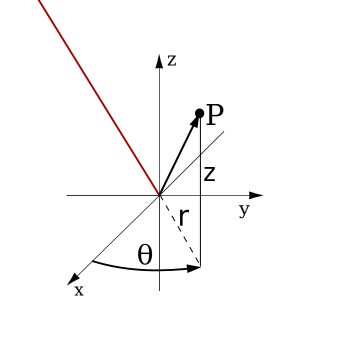
\includegraphics[width=.8in]{images/cylindricalcoords}}
Let $P=(x,y,z)$ be a point in space. This point lies on a cylinder of radius $r$, where the cylinder has the $z$ axis as its axis of symmetry.  The height of the point is $z$ units up from the $xy$ plane. The point casts a shadow in the $xy$ plane at $Q=(x,y,0)$.  The angle between the ray $\vec{OQ}$ and the $x$-axis is $\theta$.
\begin{enumerate}
\item Explain why $x=r\cos\theta$, $y=r\sin\theta$, and $z=z$.
\item What are bounds on $r$, $\theta$, and $z$ that will give all points on the surface of a cylinder of radius 1 wrapped around the $z$ axis between the $xy$ plane and $z=1$?  [Hint: the bounds on $r$ are $r=1$.]
\item What are bounds on $r$, $\theta$, and $z$ that will give all points inside a solid cylinder of radius 2 wrapped around the $z$-axis extending from 1 unit below the $xy$ plane to 1 unit above the $xy$ plane?
\end{enumerate}
\end{problem}

\begin{problem} \marginparbmw{See page 897.}\larsonfive{\marginpar{See
      Larson 11.7.}} \marginpar{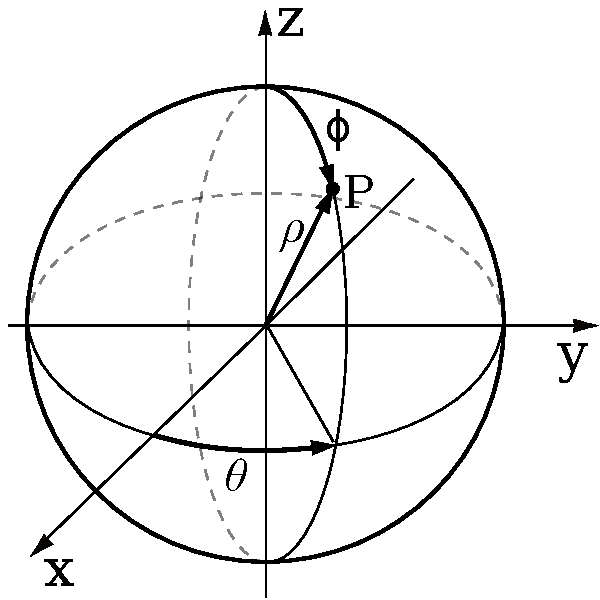
\includegraphics[width=1in]{images/sphericalcoords}
}\label{derive spherical coordinates}%
 Let
  $P=(x,y,z)$ be a point in space. This point lies on a sphere of
  radius $\rho$ (``rho''), where the sphere's center is at the origin
  $O=(0,0,0)$. The point casts a shadow in the $xy$ plane at
  $Q=(x,y,0)$.  The angle between the ray $\vec{OQ}$ and the $x$-axis
  is $\theta$, and is called the azimuth angle. The angle between
  the ray $\vec{OP}$ and the $z$ axis is $\phi$ (``phi''), and is
  called the inclination angle, polar angle, or zenith angle.

  \begin{enumerate}
  \item Explain why $x=\rho\sin\phi\cos\theta$, $y=\rho\sin\phi\sin\theta$, and $z=\rho\cos\phi$.
  \item What are bounds for $\rho$, $\theta$, and $\phi$ that will give all the points on the surface a sphere of radius 1? [Hint: the bounds for $\rho$ are $\rho=1$.]
  \item What are bounds on $\rho$, $\theta$, and $\phi$ that will give all the points on or above the $xy$ plane inside a solid sphere of radius 1?
  \item What are bounds on $\rho$, $\theta$, and $\phi$ that will give all the points on the surface of a sphere of radius 2 above the plane $z=1$ and where the $y$ coordinates are positive?
  \end{enumerate}
\end{problem}

\marginpar{See the
  \href{http://en.wikipedia.org/wiki/Spherical_coordinate_system}{Wikipedia}
  or
  \href{http://mathworld.wolfram.com/SphericalCoordinates.html}{MathWorld}
  for a discussion of conventions in different disciplines.}%
There is some disagreement between different fields about the notation
for spherical coordinates.  In some fields (like physics), $\phi$
represents the azimuth angle and $\theta$ represents the inclination
angle.  In some fields, like geography, instead of the inclination angle, the
\emph{elevation} angle is given---the angle from the $xy$-plane (lines
of lattitude are from the elevation angle).
Additionally, sometimes the coordinates are written in a different
order.  You should always check the notation for spherical coordinates
before communicating using them.
%%%%%%%%%%%%%%%%%%%%%%%%%%%%%%%%%%%%%%%%%%%%%%%%%%%%%




\begin{problem}\label{graphing spherical coordinates}%
\larsonfive{\marginpar{See Larson 11.7:89--94, 111--114.}}%
 Consider the spherical coordinates transformation 
\bmw{$$\vec T(\rho,\phi,\theta)=(\rho\sin\phi\cos\theta,\rho\sin\phi\sin\theta,\rho\cos\phi),$$ }
\larsonfive{$$\vec T(\rho,\theta,\phi)=(\rho\sin\phi\cos\theta,\rho\sin\phi\sin\theta,\rho\cos\phi),$$ }

  Graphing this transformation requires $3+3=6$ dimensions. In this problem we'll construct parts of this graph by graphing various surfaces. We did something similar for the polar coordinate transformation in problem \ref{polar coordinate transformation graph}. 
\begin{enumerate}
 \item% 
   \marginpar{See \href{https://sagecell.sagemath.org/?z=eJxVjsEKhDAMRO9-xeCpKTmId__C-1JEaEBtaPP_bLMirLe8ecOQNdRcGJqFYXm3RFjgWWxyhR5T3EoLt2K8hB__wosuaNAql2FcfWiZCdJGxkODpprO3apsHz2KhUcw7jnGxJijiie_zzp3oi_jZjWn}{Sage} or 
\href{http://www.wolframalpha.com/input/?i=parametric+plot+3d+\%282+sin+phi+cos+theta\%2C+2+sin+phi+sin+theta\%2C+2+cos+phi\%29}{Wolfram Alpha}.}%
Graph the surface $T(2,\theta,\phi)$ (in other words, the surface $\rho=2$) where $\theta\in [0,2\pi]$, $\phi\in [0,\pi]$.
 \item % 
\marginpar{See 
\href{https://sagecell.sagemath.org/?z=eJxVjrEKwzAMRPd8xZHJMioNTdf8RfZiQsCCNha2_p9WyeJuuveOQ2uouTA0C8PybomwwFlscoQfpriVFi7F-BN-9MKLLmjQKodhXD0uKvcnQdrI6MCgqabPblW2l76Lhc4xrl3GxHhEFSfnn7eZMRN9AfBbOD8}{Sage} or 
\href{http://www.wolframalpha.com/input/?i=parametric+plot+3d+\%28rho+sin+\%28pi\%2F4\%29+cos+theta\%2C+rho+sin+\%28pi\%2F4\%29+sin+theta\%2C+rho+cos+\%28pi\%2F4\%29\%29+}{Wolfram Alpha}.}%
Graph $T(\rho,\theta,\pi/4)$ for $\rho\geq 0$, $\theta\in [0,2\pi]$ (in other words, all points where $\phi=\pi/4$).  What happens if $\rho$ can be negative (i.e., $\rho\in\mathbb{R}$)?
\item Graph $T(\rho, \theta, \pi/2)$ for $\rho\in\mathbb{R}$, $\theta\in [0,2\pi]$ (in other words, all points where $\phi=\pi/2$).
 \item Graph $T(\rho,\pi/4, \phi)$ for $\rho\geq 0$, $\phi\in [0,\pi]$ (in other words, all points where $\theta=\pi/4$).
\end{enumerate}

\end{problem}




\note{Take a good look at whether we want to just incorporate these problems into the material above...}

\section{Constructing Functions}
We now know how to draw a vector field provided someone tells us the equation. How do we obtain an equation of a vector field? The following problem will help you develop the gravitational vector field.

\begin{problem}[Radial fields]
\marginpar{Use \href{https://sagecell.sagemath.org/?z=eJxz06jQqdSp0lSwVdAA0joVmlwFOfkl8WWpySX5RfFpmak5KcYpGm46CkCFusY6xpo6IIUQlkYVhKEJAOGFExs}{Sage} to plot your vector fields.  \bmw{See 16.2: 39-44 for more practice.}}%
\larsonfive{\marginpar{See Larson 15.1:1--19.}}%
Do the following:
\begin{enumerate}
 \item Let $P=(x,y,z)$ be a point in space.  At the point $P$, let $\vec F(x,y,z)$ be the vector which points from $P$ to the origin.  Give a formula for $\vec F(x,y,z)$.
 \item Give an equation of the vector field where at each point $P$ in the plane, the vector $\vec F_2(P)$ is a unit vector that points towards the origin.
 \item Give an equation of the vector field where at each point $P$ in the plane, the vector $\vec F_3(P)$ is a vector of length 7 that points towards the origin.
 \item Give an equation of the vector field where at each point $P$ in the plane, the vector $\vec G(P)$ points towards the origin, and has a magnitude equal to $1/d^2$ where $d$ is the distance to the origin.
\end{enumerate}
\end{problem}

If someone gives us parametric equations for a curve in the plane, we know how to draw the curve.  How do we obtain parametric equations of a given curve? In problem \ref{parametric curve in plane example}, we were given the parametric equation for the path of a horse, namely $x=2\cos t, y=3 \sin t$ or $\vec r(t)=(2\cos t,3\sin t)$. From those equations, we drew the path of the horse, and could have written a Cartesian equation for the path. How do we work this in reverse, namely if we had only been given the ellipse $\ds\frac{x^2}{4}+\frac{y^2}{9}=1$, could we have obtained parametric equations $\vec r(t)=(x(t),y(t))$ for the curve?

\begin{problem}\label{parameterizing plane curves}
\marginpar{Use \href{https://sagecell.sagemath.org/?z=eJwrsS1LLNJQL1HX5CpILErMTS0pykyOL8jJL9GINtJKzi_WKNHUUTDWKs7MA7JidRQ0SnQMdIy0CjI1NQFWdRJT}{Sage} or \href{http://wolfr.am/wAkR8l}{Wolfram Alpha} %http://www.wolframalpha.com/input/?i=parametric+plot+%282+cos+t,+3+sin+t%29
to visualize your parameterizations.
}%
 Give a parametrization of the top half of the ellipse $\ds\frac{x^2}{a^2}+\frac{y^2}{b^2}=1$, so $y\geq 0$.
 You can write your parametrization in the vector form $\vec r(t)=(?,?)$, or in the parametric form $x=?,\ y=?$. 
 Include bounds for $t$. 
 [Hint: Review \ref{parametric curve in plane example}.]
\end{problem}


\begin{problem}
 Give a parametrization of the straight line from $(a,0)$ to $(0,b)$. 
 You can write your parametrization in the vector form $\vec r(t)=(?,?)$, or in the parametric form $x=?,\ y=?$. 
 Remember to include bounds for $t$. [Hint: Review \ref{first line between two points} and \ref{line equation to refer to}.]
\end{problem}


\begin{problem}
 Give a parametrization of the parabola $y=x^2$ from $(-1,1)$ to $(2,4)$. 
 Remember the bounds for $t$.
\end{problem}


\begin{problem}
 Give a parametrization of the function $y=f(x)$ for $x\in[a,b]$.
 You can write your parametrization in the vector form $\vec r(t)=(?,?)$, or in the parametric form $x=?,\ y=?$. 
 Include bounds for $t$.
\end{problem}




%%%%%%%%%%%%%%%%%%%%%%%%%%%%%%%%%%%%%%%
%%%%%%%%%%%%%%%%%%%%%%%%%%%%%%%%%%%%%%%
%%%%%%%%%%%%%%%%%%%%%%%%%%%%%%%%%%%%%%%
\note{Idea.  They did the problem below already when drawing spherical coordinates.  They already practiced removing a variable.  I somehow need to make that connect to this part. How to do it, I'm not sure. Think about it, and try something different next time.}
%%%%%%%%%%%%%%%%%%%%%%%%%%%%%%%%%%%%%%%
%%%%%%%%%%%%%%%%%%%%%%%%%%%%%%%%%%%%%%%
%%%%%%%%%%%%%%%%%%%%%%%%%%%%%%%%%%%%%%%
If someone gives us parametric equations for a surface, we can draw the surface. This is what we did in problems \ref{parametric surface example} and \ref{second parametric surface example}. 
How do we work backwards and obtain parametric equations for a given surface?
This requires that we write an equation for $x$, $y$, and $z$ in terms of two input variables (see \ref{parametric surface example} and \ref{second parametric surface example} for examples). 
In vector form, we need a function $\vec r\colon \mathbb{R}^2\to\mathbb{R}^3$. 
We can often use a coordinate transformation $\vec T\colon \mathbb{R}^3\to\mathbb{R}^3$ to obtain a parametrization of a surface. 
The next three problems show how to do this.   
\begin{problem}\label{3d parametric plot}
\marginpar{Use \href{https://sagecell.sagemath.org/?z=eJwL0ajQqdSp0lSwVYCyuAqKMvNKFJRCNKpsK7QrNRUyi5V0FGA8roLEosTc1JKizOT4gpz8Eg2YhA5Iv66xjjGIVQlhaQIALhka5w}{Sage} or
\href{http://wolfr.am/zk2KTu}{Wolfram Alpha} %http://www.wolframalpha.com/input/?i=parametric+plot+3d+%28x%2Cy%2Cx%2By%29
to plot your parametrization.  \bmw{See 16.5: 1-16 for more practice.}}%
\larsonfive{\marginpar{See Larson 15.5:21--30 and 15.5, Example 3.}}%
 Consider the surface $z=9-x^2-y^2$ plotted in problem \ref{surface graph for a function of two variables}.
\begin{enumerate}
 \item 
Using the rectangular coordinate transformation $\vec T(x,y,z)=(x,y,z)$, give a parametrization $\vec r\colon \mathbb{R}^2\to\mathbb{R}^3$ of the surface. 

This is the same as saying $$x=x, y=y, z=?.$$
[Hint: Use the surface equation to eliminate the input variable $z$ in $T$.]

 \item What bounds must you place on $x$ and $y$ to obtain the portion of the surface above the plane $z=0$?
 \item If $z=f(x,y)$ is any surface, give a parametrization of the surface (i.e., $x=?, y=?, z=?$ or $\vec r (?,?)=(?,?,?)$.)
\end{enumerate}

\end{problem}
\begin{problem}%
\marginpar{Use \href{https://sagecell.sagemath.org}{Sage} or \href{http://wolframalpha.com}{Wolfram Alpha} to plot your parametrization with your bounds (see \ref{3d parametric plot} for examples).  \bmw{See 16.5: 1-16 for more practice.}}%
\larsonfive{\marginpar{See Larson 15.5:1--10}}%
 Again consider the surface $z=9-x^2-y^2$.
\begin{enumerate}
 \item
Using cylindrical coordinates, $\vec T(r,\theta,z) = (r\cos \theta, r\sin\theta, z)$, obtain a parametrization $\vec r(r,\theta)=(?,?,?)$ of the surface using the input variables $r$ and $\theta$. In other words, if we let $x=r\cos \theta, y=r\sin\theta, z=z$, write $z=9-x^2-y^2$ in terms of $r$ and $\theta$.
 \item What bounds must you place on $r$ and $\theta$ to obtain the portion of the surface above the plane $z=0$?
\end{enumerate}

\end{problem}


\note{probably just delete this next problem, since we did similar things above}

\begin{problem}%
\marginpar{We did very similar things in problem \ref{graphing spherical coordinates}.}%
\bmw{\marginpar{See 16.5: 1-16 for more practice.}}%
\larsonfive{\marginpar{See Larson 15.5:1--10}}%
Recall the spherical coordinate transformation 
\bmw{$$\vec T(\rho,\phi,\theta) = (\rho\sin\phi\cos \theta, \rho\sin\phi\sin \theta,\rho \cos \phi).$$ }%
\larsonfive{$$\vec T(\rho,\theta, \phi) = (\rho\sin\phi\cos \theta, \rho\sin\phi\sin \theta,\rho \cos \phi).$$}%
This is a function of the form $\vec T\colon \mathbb{R}^3\to\mathbb{R}^3$.  If we hold one of the three inputs constant, then we have a function of the form $\vec r\colon \mathbb{R}^2\to\mathbb{R}^3$, which is a parametric surface.
\begin{enumerate}
 \item \marginpar{Use \href{https://sagecell.sagemath.org}{Sage} or \href{http://www.wolframalpha.com/}{Wolfram Alpha} to plot each parametrization (see \ref{3d parametric plot} for examples).}%
Give a parametrization of the sphere of radius 2, using $\phi$ and $\theta$ as your input variables. 
 \item Give a set of bounds on $\phi$ and $\theta$ that will hit every point on the sphere.
 \item What bounds should you place on $\phi$ and $\theta$ if you only want the portion of the sphere above the plane $z=1$?
\end{enumerate}
\end{problem}

Sometimes you'll have to invent your own coordinate system when constructing parametric equations for a surface.  If you notice that there are lots of circles parallel to one of the coordinate planes, try using a modified version of cylindrical coordinates. Instead of circles in the $xy$ plane ($x=r\cos\theta,y=r\sin\theta,z=z$), maybe you need circles in the $yz$-plane ($x=x,y=r\cos\theta,z=r\sin\theta$) or the $xz$ plane.  Just look for lots of circles, and then construct your parametrization accordingly.
\begin{problem}
\larsonfive{\marginpar{See Larson 15.5:21--30.}}%
Find parametric equations for the surface $x^2+z^2=9$. [Hint: read the paragraph above.]  
\begin{enumerate}
 \item\marginpar{Use \href{https://sagecell.sagemath.org}{Sage} or \href{http://www.wolframalpha.com/}{Wolfram Alpha} to plot each parametrization  (see \ref{3d parametric plot} for examples).}%
 What bounds should you use to obtain the portion of the surface between $y=-2$ and $y=3$?
 \item What bounds should you use to obtain the portion of the surface above $z=0$?
 \item What bounds should you use to obtain the portion of the surface with $x\geq 0$ and $y\in[2,5]$?
\end{enumerate}
\end{problem}

\bmw{\begin{problem}
 Construct a graph of the surface $z = x^2-y^2$.  Do so in 2 ways.  (1) Construct a 3D surface plot.  (2) Construct a contour plot, which is a graph with several level curves. Which level curve passes through the point $(3,4)$? 
 Use Wolfram Alpha to know if you're right.  Just type ``plot z=x\^2-y\^2.''
\end{problem}

\begin{problem}
Construct a plot of the vector field $$\vec F(x,y) = (x+y, -x+1)$$ by graphing the field at many integer points around the origin (I generally like to get the 8 integer points around the origin, and then a few more).
Then explain how to modify your graph to obtain a plot of the vector field $$\hat F(x,y) = \frac{(x+y, -x+1)}{\sqrt{(x+y)^2+(1-x)^2}}.$$ 
\end{problem}}


%%% Local Variables: 
%%% mode: latex
%%% TeX-master: "215-problems"
%%% End: 
